\section{Licenze software}

\subsection*{Materiale di riferimento}

\begin{itemize}

\item \textit{Understanding Open Source and Free Software Licensing} - Andrew Laurent;
\item \textit{Open Source Licensing: Software freedom and intellectual property law}.

\end{itemize}

\subsection{Capisaldi}

Il diritto d'autore arriva fino a 70 anni dopo la morte. Al giorno d'oggi in realtà la grande maggioranza dei libri hanno un utilità che dura pochi anni da quando sono stati prodotti, a meno che non sia un grande classico o un best-seller. La protezione è espressa sotto forma percepibile, dev'essere qualcosa che uno ``ha creato''. Inoltre non c'è nessuna registrazione necessaria per avere il diritto d'autore. Un discorso a parte è il \textbf{work for hire}, ovvero quando qualcuno produce un'opera lavorando per qualcun altro. Quando si lavora come dipendenti, a meno di clausole particolari, tutto ciò che si produce è proprietà del datore di lavoro, viene ceduta la proprietà intellettuale del proprio lavoro all'azienda.  

Una cosa che vedremo molto spesso sono le \textbf{garanzie}, perchè ogni copyright, soprattutto quelli open source, hanno una clausola che il più possibile cerca di raggiungere una certa forma di garanzia, in modo da non dover andare incontro a problematiche. Ci sono due tipi di garanzie:

\begin{itemize}

\item \textbf{Garanzie esplicite}, sono quelle che io do esplicitamente per cercare di rendere più appetibile la mia vendita; 

\item \textbf{Garanzie implicite}, che di fatto sono ``forzate'' dalla legge; esempio garanzie di commerciabilità sui prodotti acquistati, o quelle di idoneità a un certo scopo.

\end{itemize}

\subsection{X License (MIT license)}

È la licenza più basilare, licenza originale di X Windows. Essenzialmente permette di \textit{fare tutto}, libertà di modifica, di copia, di ridistribuzione del software. Il codice sorgente può essere redistribuito liberamente, senza restrizioni sul formato (ad esempio si può scegliere di redistribuirlo solo in forma binaria). Quello che è necessario è \textbf{mantenere la licenza originale}, in modo che la persona possa vedere la licenza con la quale è stato prodotto quel software. Ci sono naturalmente delle clausole di salvaguardia. 	

\begin{lstlisting}[caption=Licenza MIT]

Copyright (c) <year> <copyright holders>

Permission is hereby granted, free of charge, to any person
obtaining a copy of this software and associated documentation
files (the ``Software''), to deal in the Software without
restriction, including without limitation the rights to use,
copy, modify, merge, publish, distribute, sublicense, and/or sell
copies of the Software, and to permit persons to whom the
Software is furnished to do so, subject to the following
conditions:

The above copyright notice and this permission notice shall be
included in all copies or substantial portions of the Software.

THE SOFTWARE IS PROVIDED ``AS IS'', WITHOUT WARRANTY OF ANY KIND,
EXPRESS OR IMPLIED, INCLUDING BUT NOT LIMITED TO THE WARRANTIES
OF MERCHANTABILITY, FITNESS FOR A PARTICULAR PURPOSE AND
NONINFRINGEMENT. IN NO EVENT SHALL THE AUTHORS OR COPYRIGHT
HOLDERS BE LIABLE FOR ANY CLAIM, DAMAGES OR OTHER LIABILITY,
WHETHER IN AN ACTION OF CONTRACT, TORT OR OTHERWISE, ARISING
FROM, OUT OF OR IN CONNECTION WITH THE SOFTWARE OR THE USE OR
OTHER DEALINGS IN THE SOFTWARE.

\end{lstlisting}

L'obiettivo è quello di \textbf{proteggere} chi ha scritto software sotto questa licenza, ecco perchè ci sono tutta una serie di garanzie, in questo modo si evitano problemi futuri dovuti alla redistribuzione. Qualunque tipo di garanzia possibile è \textbf{coperta}, anche se non sempre queste clausole sono valide, ad esempio potrebbero non essere validi in alcuni paesi. Ad ogni modo, nonostante queste garanzie, è una licenza che risulta comunque molto permissiva. 

\subsection{Licenze BSD}

Sono leggermente più restrittive rispetto alla licenza MIT. In realtà ce ne sono diverse:

\begin{itemize}

\item BDS a 4 clausole;
\item BSD a 3 clausole;
\item BSD a 2 clausole.

\end{itemize}

Storicamente si sono sviluppate in ordine decrescente, man mano hanno tolto una clausola perchè sostanzialmente creava dei problemi. La licenza BSD a quattro clausole si è dimostrata infatti inutilizzabile nella pratica, perchè diveniva ingestibile tenere conto di tutti gli autori del software. 

\subsubsection{BDS a due clausole}

È la licenza di \textbf{NetBSD} e di fatto corrisponde alla MIT license, con l'aggiunta dell'obbligo di inserire la documentazione anche nella redistribuzione.

\begin{lstlisting}[caption=BSD a due clausole (NetBDS)]


Copyright (c) 2008 The NetBSD Foundation, Inc.
All rights reserved.

This code is derived from software contributed to The NetBSD Foundation
 by 

Redistribution and use in source and binary forms, with or without
modification, are permitted provided that the following conditions
are met:
 1. Redistributions of source code must retain the above copyright
    notice, this list of conditions and the following disclaimer.
 2. Redistributions in binary form must reproduce the above copyright
    notice, this list of conditions and the following disclaimer in the
    documentation and/or other materials provided with the distribution.

 THIS SOFTWARE IS PROVIDED BY THE NETBSD FOUNDATION, INC. AND CONTRIBUTORS
 ``AS IS'' AND ANY EXPRESS OR IMPLIED WARRANTIES, INCLUDING, BUT NOT LIMITED
 TO, THE IMPLIED WARRANTIES OF MERCHANTABILITY AND FITNESS FOR A PARTICULAR
 PURPOSE ARE DISCLAIMED.  IN NO EVENT SHALL THE FOUNDATION OR CONTRIBUTORS
 BE LIABLE FOR ANY DIRECT, INDIRECT, INCIDENTAL, SPECIAL, EXEMPLARY, OR
 CONSEQUENTIAL DAMAGES (INCLUDING, BUT NOT LIMITED TO, PROCUREMENT OF
 SUBSTITUTE GOODS OR SERVICES; LOSS OF USE, DATA, OR PROFITS; OR BUSINESS
 INTERRUPTION) HOWEVER CAUSED AND ON ANY THEORY OF LIABILITY, WHETHER IN
 CONTRACT, STRICT LIABILITY, OR TORT (INCLUDING NEGLIGENCE OR OTHERWISE)
 ARISING IN ANY WAY OUT OF THE USE OF THIS SOFTWARE, EVEN IF ADVISED OF THE
 POSSIBILITY OF SUCH DAMAGE.

 \end{lstlisting}

 Essenzialmente si può pensarla come una licenza BSD in cui nella distribuzione in forma binaria bisogna mantenere tutta la documentazione e la licenza. 

 \subsubsection{BSD a tre clausole}

 La BSD a tre clausole ha un'impostazione un po' più innovatoria. Si tratta comunque di una licenza molto ``generosa'', non sono per nulla invasive. Comprende le due clausole precedenti più la seguente:

 \begin{lstlisting}[caption=BSD a tre clausole]

3. Neither the name of the <organization> nor the
   names of its contributors may be used to endorse or promote products
   derived from this software without specific prior written permission.

\end{lstlisting} 

In pratica permette di ``fare quello che si vuole'' però non è possibile farsi pubblicità usando il nome del copyright holder a meno che non si abbia un permesso. Ad esempio non si può dire ``il mio software è più sicuro perchè è sotto licenza BSD''. È una delle licenze più comuni nei sistemi BSD, non crea nessun problema, ed è approvata dalla OSI.

\subsubsection{BSD a quattro clausole}

Ma la licenza originale di BSD unix aveva un'altra clausola che era molto più invasiva. Aveva le stesse clausole già viste, in più:

\begin{lstlisting}[caption=BSD a quattro clausole] 

4. All advertising materials mentioning features or use of this software
   must display the following acknowledgement:
   This product includes software developed by the <organization>.

\end{lstlisting}

Chiaramente questo valeva per tutti gli autori e le entità che avevano donato il codice, quindi diventava un po' problematico riportarli tutti, tanto è vero che non è stata approvata dalla OSI. Un problema più serio è che non è compatibile con la GPL perchè questa clausola aggiuntiva non è prevista dalla GPL. Quindi se si voleva cambiare la licenza del prodotto a GPL si riscontravano grossi problemi in quanto si dovrebbe togliere questa clausola. Da un punto di vista pratico era inoltre molto problematico dover tener traccia di tutti gli autori (gli indirizzi email per esempio possono cambiare nel tempo).

\subsection{Apache license}

La Licenza Apache è una licenza di software libero non copyleft scritta dalla \textbf{Apache Software Foundation} (ASF) che obbliga gli utenti a preservare l'informativa di diritto d'autore e d'esclusione di responsabilità nelle versioni modificate.

Come ogni licenza di software libero, la licenza Apache consente agli utenti di usare il software per ogni scopo, di distribuirlo, modificarlo e di distribuire versioni modificate del software.

La licenza Apache non richiede che versioni modificate del software siano distribuite secondo i termini della stessa licenza o come software libero, richiede solo che si includa un'informativa del fatto che si è utilizzato software licenziato secondo i termini della Licenza Apache.

Quindi, a differenza di quanto accade con le licenze copyleft, gli utenti di versioni modificate del software licenziato secondo i termini della Licenza Apache non godono necessariamente delle suddette libertà o, considerando la situazione dal punto di vista del licenziatario, esso ha la libertà di utilizzare il software in ogni modo, anche in prodotti proprietari, a danno degli utilizzatori (vedi l'articolo 4).

\subsubsection{Versioni}

Ci sono state tutta una serie di versioni di questa licenza, che è cambiata dalla 1.0 fino alla 2.0. La \textbf{1.0} era una BSD a quattro clausole più una clausola di rinomina, che essenzialmente diceva che se si prendeva un prodotto che utilizzava del codice di Apache era necessario chiamare il prodotto in modo diverso da Apache. Questa clausola voleva ottenere l'effetto di evitare che il codice sorgente di Apache fosse la base di una miriade di web server diversi che utilizzavano quel codice lì, volevano evitare una frammentazione eccessiva, perchè sarebbe stato un danno per la comunità. 

Nella versione \textbf{1.1} hanno modificato queste cose, hanno tolto la quarta clausola di BSD, la clausola di rinomina è rimasta, e hanno aggiunto una clausola pubblicitaria sulla documentazione; in pratica era necessario pubblicizzare nella documentazione il fatto che il codice si basasse sul prodotto Apache. 

\begin{lstlisting}[caption=licenza Apache 1.1]

 ====================================================================
 The Apache Software License, Version 1.1

 Copyright (c) 2000 The Apache Software Foundation.  All rights
 reserved.

 Redistribution and use in source and binary forms, with or without
 modification, are permitted provided that the following conditions
 are met:

 1. Redistributions of source code must retain the above copyright
    notice, this list of conditions and the following disclaimer.

 2. Redistributions in binary form must reproduce the above copyright
    notice, this list of conditions and the following disclaimer in
    the documentation and/or other materials provided with the
    distribution.

 3. The end-user documentation included with the redistribution,
    if any, must include the following acknowledgment:
       "This product includes software developed by the
        Apache Software Foundation (http://www.apache.org/)."
    Alternately, this acknowledgment may appear in the software itself,
    if and wherever such third-party acknowledgments normally appear.

 4. The names "Apache" and "Apache Software Foundation" must
    not be used to endorse or promote products derived from this
    software without prior written permission. For written
    permission, please contact apache@apache.org.

 5. Products derived from this software may not be called "Apache",
    nor may "Apache" appear in their name, without prior written
    permission of the Apache Software Foundation.

 THIS SOFTWARE IS PROVIDED ``AS IS'' AND ANY EXPRESSED OR IMPLIED
 WARRANTIES, INCLUDING, BUT NOT LIMITED TO, THE IMPLIED WARRANTIES
 OF MERCHANTABILITY AND FITNESS FOR A PARTICULAR PURPOSE ARE
 DISCLAIMED.  IN NO EVENT SHALL THE APACHE SOFTWARE FOUNDATION OR
 ITS CONTRIBUTORS BE LIABLE FOR ANY DIRECT, INDIRECT, INCIDENTAL,
 SPECIAL, EXEMPLARY, OR CONSEQUENTIAL DAMAGES (INCLUDING, BUT NOT
 LIMITED TO, PROCUREMENT OF SUBSTITUTE GOODS OR SERVICES; LOSS OF
 USE, DATA, OR PROFITS; OR BUSINESS INTERRUPTION) HOWEVER CAUSED AND
 ON ANY THEORY OF LIABILITY, WHETHER IN CONTRACT, STRICT LIABILITY,
 OR TORT (INCLUDING NEGLIGENCE OR OTHERWISE) ARISING IN ANY WAY OUT
 OF THE USE OF THIS SOFTWARE, EVEN IF ADVISED OF THE POSSIBILITY OF
 SUCH DAMAGE.
 ====================================================================

 This software consists of voluntary contributions made by many
 individuals on behalf of the Apache Software Foundation.  For more
 information on the Apache Software Foundation, please see
 <http://www.apache.org/>.

 Portions of this software are based upon public domain software
 originally written at the National Center for Supercomputing Applications,
 University of Illinois, Urbana-Champaign.

\end{lstlisting}

L'Apache 1.1 non è durata molto, in quanto è subentrata poi l'Apache \textbf{2.0}, che cambia completamente. Mentre dalla 1.0 alla 1.1 hanno cambiato un po' di clausole, con la 2.0 ci sono cambiamenti molto grandi, ed è la prima licenza che analizziamo che affronta il \textbf{problema dei brevetti}. L'idea fondamentale dell'Apache 2.0 è di affrontare il problema dei brevetti. La questione è che le licenze software libere erano state formate in un momento in cui la proprietà intellettuale significava copyright. Questo non era più vero, piano piano era divenuta sempre più pressante il \textbf{problema dei brevetti}. Non si è infatti obbligati a fornire delle licenze per i brevetti, è a discrezione del proprietario. Anche dentro Apache si sono posti dunque il problema di evitare che qualcuno potesse crearsi il proprio web server che aveva tutte le funzionalità di Apache, aggiungergi delle proprie funzionalità (algoritmi) delle quale possedeva i brevetti e reimmettere nel mercato questa nuova versione. Si impose dunque una clausola sui brevetti, in cui quando una persona contribuiva ad Apache forniva anche i propri brevetti. Era necessario di distinguere il concetto di \textbf{modifica} da quello di \textbf{contribuzione}. Si pensa al modello in cui c'è uno \textbf{sviluppo centralizzato}.	
\linebreak
\linebreak
I due files che devono essere inclusi nella directory principale dei prodotti software distribuiti sono:

\begin{itemize}

\item \textbf{LICENSE} - una copia della licenza.
\item \textbf{NOTICE} - un'``informativa'' testuale che elenca i nomi delle librerie licenziate che sono utilizzate, con i nomi degli sviluppatori. Nel codice redistribuito si deve preservare in ogni file licenziato qualsiasi informativa di diritto d'autore e di brevetti presente ed in ogni file modificato si deve aggiungere un'informativa specificando che il file è stato modificato.

\end{itemize}

\begin{lstlisting}[caption=licenza Apache 2.0]

Copyright [yyyy] [name of copyright owner]

Licensed under the Apache License, Version 2.0 (the "License");
you may not use this file except in compliance with the License.
You may obtain a copy of the License at

    http://www.apache.org/licenses/LICENSE-2.0

Unless required by applicable law or agreed to in writing, software
distributed under the License is distributed on an "AS IS" BASIS,
WITHOUT WARRANTIES OR CONDITIONS OF ANY KIND, either express or implied.
See the License for the specific language governing permissions and
limitations under the License.

\end{lstlisting}

\subsubsection{Filosofia delle licenze BSD}

Le licenze BSD sono fatte per permettere gli sfruttamenti proprietari. Vanno ovviamente nella direzione opposta di quella del mondo del software libero. In genere queste licenze ci sono quando si vuole creare uno standard, ma devono essere consistenti con l'obiettivo dei progetti che le scelgono (esempio X, BSD unix). Questo favorisce la massima diffusione del codice (originale o derivato). Le licenze copyleft hanno come obiettivo invece quello di impedire gli sfruttamenti proprietari. Non si può modificare la licenza in modo proprietario. 

\subsection{GPL v2}

\subsubsection{Le basi}

La licenza GPL permette la libera copia non modificata, a patto di mantenere le licenze e le clausole di salvaguardia intatte. I prodotti derivati devono essere essi stessi sotto GPL. Questa è la base, ma in verità è una licenza che è stata molto modificata negli anni. La prima cosa che uno potrebbe fare e prendere il programma e distribuirlo (copiarlo), purchè mantenga le licenze e la clausole. Diverso è se io prendo la distribuzione dei sorgenti e li modifico. In questo caso la GPL prevede tutta una serie di clausole sia per la tutela dell'autore originale del software che per gli stessi utenti finali di quel software. L'obbligo è di inserire in ogni singolo file modificato degli avvisi di modifica, spesso nell'intestazione del codice, in modo che chiunque possa vedere quali modifiche sono state fatte, in modo che se sorgono problemi sia identificabile il responsabile. La seconda cosa che si deve fare è mettere il risultato finale sotto GPL. Per sorgenti si intende i file che vengono compilati, gli script utilizzati e il software che viene utilizzato (ad esempio compilatori, dipendenze varie, ...). Un'ulteriore clausola è che eventuali avvisi interattivi sulla licenza devono rimanere. Per esempio ci sono alcuni programmi che quando vengono lanciati mostrano un \textit{pop-up}, o degli avvisi con alcune informazioni, ad esempio le clausole di salvaguardia. Questo deve rimanere. 

\subsubsection{Restrizione sulla distribuzione di binari}

Maggiori restrizioni vi sono sulla modifica e redistribuzione dei file binari. Essi devono obbligatoriamente essere \textbf{accompagnati dai relativi file sorgenti}. L'accesso ai file sorgenti dev'essere libero, senza penalizzazioni. La seconda opzione è di fornire un'offerta scritta in cui ognuno può ottenere i sorgenti per almeno tre anni. L'offerta scritta ha chiaramente un costo, nel momento in cui io mando il cd con i sorgenti a qualcuno devo poter farlo pagare, quindi sostanzialmente faccio pagare la spedizione, il che non comporta costi eccessivi. La terza possibilità consiste nell'informare dove stanno i file sorgenti (sul web presumibilmente), dove poterli prelevare. Questo è possibile solamente per distribuzioni non commerciali.  

\subsubsection{Cosa sono i sorgenti?}

È chiaro che senza una \textbf{definizione formale} di cosa siano i file sorgente si fa presto a incappare in errori. Tutto quello che in qualche modo \textit{interagisce} con il programma dev'essere fornito sotto GPL. 

\begin{itemize}

\item Sorgenti per tutti i \textbf{moduli} del programma;

\item Tutti gli \textbf{script} e tutto quanto necessario per la compilazione, ad esempio \textit{Makefile}, parser, linker, compilatori aggiuntivi, ... In sostanza tutto ciò che serve per far partire il programma;

\item \textbf{Eccezione} di quanto normalmente distribuito con il nucleo del sistema operativo. L'idea era: uno compila sotto ambiente Microsoft, usando il suo Visual C++ o altro che fa parte del sistema operativo, di quello cose allora non deve distribuire il binario. Non era molto chiara come clausola, non si capiva fin dove bisognava arrivare.
 
\end{itemize}

Una clausola importante è stata istituita per risolvere il problemi del rapporto tra autore originale e utilizzatore finale: chi riceve una copia del sorgente ottiene anche una \textbf{licenza d'uso} anche dal concessore originale. Automaticamente si è in grado di punire ogni violazione, se si è interessati a farlo. Chiaramente non risolve completamente il problema perchè non tutto il grafo di distribuzione è in grado di perseguire una violazione, solamente la sotto-catena che va dal distributore originale a quello finale; ma quello che conta è l'autore originale che detiene gran parte dell'interesse sul prodotto. In questo modo si evitava che qualcuno prendesse del software da uno sviluppatore ``piccoletto'' che a quel punto sarebbe stato tagliato fuori. 
\linebreak
\linebreak
Un'ulteriore clausola è quella della cosiddetta \textit{``libertà o morte''}, pensata soprattutto per i brevetti; già allora c'era la consapevolezza che il problema dei brevetti era importante. Questa clausola dice essenzialmente che se si distribuisce un software però vi sono altre cause esterne che impediscono i diritti allora il software non può essere distribuito. Ad esempio se una legge impedisce di distribuire il codice sorgente, l'intero software protetto da GNU GPLv2 non può essere distribuito. La speranza è quella di rendere meno allettante per le imprese il ricorso alle minacce di brevetto, ovvero esigere un corrispettivo da parte degli sviluppatori di software libero.

\begin{lstlisting}[caption=Licenza GPLv2]

one line to give the program's name and an idea of what it does.
Copyright (C) yyyy  name of author

This program is free software; you can redistribute it and/or
modify it under the terms of the GNU General Public License
as published by the Free Software Foundation; either version 2
of the License, or (at your option) any later version.

This program is distributed in the hope that it will be useful,
but WITHOUT ANY WARRANTY; without even the implied warranty of
MERCHANTABILITY or FITNESS FOR A PARTICULAR PURPOSE.  See the
GNU General Public License for more details.

You should have received a copy of the GNU General Public License
along with this program; if not, write to the Free Software
Foundation, Inc., 51 Franklin Street, Fifth Floor, Boston, MA  02110-1301, USA.

/* se il programma e' interattivo:

Gnomovision version 69, Copyright (C) year name of author
Gnomovision comes with ABSOLUTELY NO WARRANTY; for details
type `show w'.  This is free software, and you are welcome
to redistribute it under certain conditions; type `show c' 
for details.

*/

Yoyodyne, Inc., hereby disclaims all copyright
interest in the program `Gnomovision'
(which makes passes at compilers) written 
by James Hacker.

signature of Ty Coon, 1 April 1989
Ty Coon, President of Vice

\end{lstlisting}

\subsubsection{LGPL v2.1}

Esiste una versione leggermente modificata della GPL, la \textbf{GNU Lesser/Library General Public License} o più semplicemente \textbf{LGPL}, pensata per le librerie. Essenzialmente mentre la GPL richiede che tutti i moduli che utilizzano quel programma vengano forniti sotto licenza GPL, la LGPL permette di più. In questo caso il progetto GNU voleva offrire una scelta, e questa scelta è stata una versione della GPL indebolita che permetta ad altri programmi di utilizzare la libreria ma allo stesso tempo non permettere che la parte GPL della libreria venisse modificata in modo proprietario. Ci sono varie clausole a questa licenza:

\begin{itemize}

\item Il software modificato dev'essere una \textbf{libreria} (anche se è una clausola non molto rispettata);
\item Bisogna fare uno sforzo ragionevole per evitare di rendere necessarie tabelle o dati esterni non distribuiti;
\item Le normali clausole della GPL.

\end{itemize}

È sempre previsto che un programma che sia sotto LGPL possa \textit{traghettare} e diventare GPL. La GPL infatti vuole poter racchiudere il massimo numero di programmi possibile sotto di essa.

La caratteristica cruciale della LGPL è la possibilità di linkare il programma con la libreria scegliendo la propria licenza, a patto che:

\begin{itemize}

\item Sia permesso il \textbf{reverse engineering}, ovvero il fatto di poter comprendere ed analizzare il programma e di poter partire da esso per sviluppare una nuova versione;
\item Sia distribuito il codice sorgente originale della libreria insieme ai file oggetto del resto del programma;
\item Oppure si utilizzi un linking dinamico.

\end{itemize}

\subsection{Filosofia delle licenze copyleft}

Passiamo ora ad analizzare le licenze copyleft pure. Essenzialmente partono con uno scopo ``sociale'', ovvero garantire la massima libertà agli utenti, agli utilizzatori. Hanno lo scopo di favorire uno \textbf{sviluppo comunitario} di molte persone e aziende che lavorano insieme su una base paritaria e con tutta una serie di garanzie in comune. Ciascuno crea e contribuisce e allo stesso tempo ha la garanzia che il resto della comunità faccia altrettanto. Un'altra ragione per la quale la GPL si è dimostrata molto buona è stata il \textbf{rapporto con le imprese}, perchè chiaramente un'azienda che distribuisce codice sotto GPL ha delle garanzie nei confronti dei concorrenti, sanno che i loro rivali non possono prendere il prodotto e farne uno proprietario senza condividere il codice, al massimo possono prendere il codice e costruire un altro prodotto GPL, ma non è molto ragionevole come idea, ben più sensato sarebbe contribuire insieme allo sviluppo: invece di fare due prodotti concorrenti ne si fa uno migliore in due, per esempio. Questa realtà sarebbe molto più difficile se l'azienda rilasciasse il prodotto sotto ad esempio licenza BSD. La GPL dà la garanzia di un \textbf{rapporto paritetico}. 

La GPL non va molto bene in alcuni settori, per esempio quando si vuole creare uno standard. Le licenze copyleft vanno bene quando si vuole creare uno sviluppo comunitario oppure quando si vuole esternalizzare una parte del proprio lavoro. 

\subsection{GPL v3}

È una licenza copyleft molto importante, fatta di recente e che presenta diverse innovazioni per il progetto GNU, il quale non aveva fino ad allora la capacità di coinvolgere una comunità attorno al proprio software. La comunità era molto debole. Bisognava cercare di creare una licenza che fosse il più comunitaria possibile la quale potesse essere discussa dalle persone. Inizialmente fu proposta una licenza iniziale. Venne poi creato un'interfaccia con la quale gli sviluppatori potevano fare proposte sulle singole linee della licenza. Era vitale capire gli interessi delle varie anime della comunità e cercare di fare il meglio per rappresentarle tutte nel miglior modo possibile. In questo modo si andava incontro a tutte le perplessità degli sviluppatori. La GPL v3 ha introdotto diverse modifiche e risolto diversi problemi della versione precedente. 

Il primo problema grosso era la \textbf{tivoizzazione}, legato alla distribuzione del \textbf{TiVo}, un apparecchio che si attacca alla TV e con il quale è possibile registrare i film in alta definizione. Questo chiaramente comporta delle problematiche per i produttori di film, dvd, ecc. Una soluzione che si cercò fu quella di impedire il trasferimento su memoria esterna dal TiVo. Il sistema operativo su cui si appoggiava il TivVo era però Linux, del quale era possibile modificare il kernel, quindi c'era la possibilità di modificare il kernel e permettere il trasferimento. A questo problema si rispose mettendo dunque un controllo nel firmware con un controllo crittografico. In questo modo se il kernel veniva modificato l'apparecchio non partiva e veniva bloccato. Questa cosa ad alcuni andava bene, ma ad altri no. Questo è stato uno dei primi momenti in cui c'è stato uno scisma fra la comunità open-source e la comunità del software libero. La comunità open-source, che è interessata principalmente al software libero come modo per favorire l'interazione con lo sviluppo di un software in modo più efficiente, non aveva grossi problemi con questo blocco per l'utilizzatore finale, dal momento che comunque il kernel era modificabile. La comunità del software libero, al contrario, non era molto permissivo su questo, percepiva il rischio di avere una tivoizzazione completa dell'hardware. Quelli erano anni in cui sempre più periferiche erano bloccate in quel modo.

L'altro problema erano due leggi: la \textbf{Digital Millenium Copyright} (\textbf{DRM}) e la \textbf{Act/European Union Copyright Directive}, due leggi create per soccombere a problemi di programmi che miravano alla sicurezza. Secondo queste leggi non era possibile e non era legale prendere un programma e modificarlo in modo da rimuovere una misura di protezione digitale (esempio firmware che impediscono i DVD copiati). Anche questo poneva un problema per la GPL.

Un terzo problema era quello legato ai \textbf{brevetti software}, problema molto grave che sussiste tuttora, anche se negli ultimi anni l'aria è un po' cambiata, anche se il problema legale c'è sempre. Il problema è che c'è la possibilità di brevettare degli algoritmi matematici, se un programma che è sotto GPL utilizza quell'algoritmo di fatto viene bloccato e non reso disponibile. Il fatto che il programma che era libero dovesse rimanere libero veniva aggirato in questo modo. Con la GPL v2 il problema dei brevetti era un problema molto sentito, ora è invece molto importante. 

La GPL v3 aveva dunque lo scopo di affrontare tutti questi problemi che la GPL v2 si era dimostrata incapace di affrontarli. 

\subsubsection{Brevetti software: la teoria}

Vediamo la legislazione corrente riguardo ai brevetti:

\begin{lstlisting}

European pattern shall be granted for any inventions which are susceptible of industrial application, which are new and which involve an intentive step.

The following in particular shall not be regrated as inventions within the meaning of paragraph 1:

  - discoveries, scientific theories and mathematical methods;
  - (b) aestethic creations;
  - (c) schemes, rules and methods for allperforming mental acts, playing games or doing business, and programs for computers;
  - (d) presentations of information.

The provisions of paragraph 2 shall exclude patentability of the subject-matter or activities referred to in that provision only to the extent to which a European patent application or European patent relates to such subject-matter or activities as such.

Methods for treatment of the human or animal body by surgery or therapy and diagnostic methods practised on the human or animal body shall not be regarded as inventions which are susceptible of industrial application not apply to products, in particular substances or compositions, for use in any of these methods.

\end{lstlisting}

\subsubsection{Brevetti software: la realtà}

\begin{lstlisting}

Disclosed is a method of implementing a preview window in an object oriented programming system that includes an application having at least a first panel and a second panel that are selectively displayable on a display screen. The second panel displays underlying information and the first panel displays an abbreviated representation of the underlying information. In the present invention, the user can temporarily display a preview window that contains undelying information while viewing the first panel.

\end{lstlisting}

Questo è un piccolo esempio di brevetto software. L'EPO ha già assegnato 3000 brevetti al software.

\subsubsection{GPL v3 e brevetti software}

I brevetti software sono un \textbf{problema} per la GPL. Il problema è che i brevetti sono molto diffusi e nel campo del software sono molto generali e tendono a coprire molte cose. Questo creava dei prodotti software che in teoria erano liberi ma che nella pratica non lo erano, magari involontariamente. Ogni software violava qualche brevetto anche senza che lo sviluppatore lo sapesse. È inoltre anche difficile consultare i brevetti che potrebbero impattare il proprio software (pensare ad esempio a dover vedersi tutti i brevetti per sviluppare un programma su Qt).

Una possibile soluzione potrebbe essere rilasciare codice libero ma protetto da brevetti, ma non è la soluzione migliore chiaramente. La soluzione si ha con la GPL v3 che afferma che quando si rilascia un programma sotto questa licenza si \textbf{concede l'uso di brevetti} utilizzati dalla propria versione del programma. Questa è una delle grosse modifiche.

\subsubsection{Tivoizzazione}

Si stavano creando delle \textbf{chiavi} che bloccavano la modifica del software e che venivano verificate (blocchi del firmware). Questo era chiaramente un problema. La soluzione la si è trovata con la GPL v3, in cui si afferma che chi distribuisce apparecchi datati di software licenziato sotto la GNU GPL v3, deve includere nella distribuzione del codice sorgente tutte le informazioni necessaire - ivi incluse per esempio le chiavi digitali necessarie - per compilare una versione del codice modificato pienamente funzionante sull'hardware distribuito. Questa cosa non si applica all'interno di dispositivi industriali in cui il fatto che nessuno possa modificare il programma è una componente importante.

\subsubsection{GPL v3 e DMCA/EUCD}

Secondo DMCA/EUCD era \textbf{illegale rimuovere una misure di protezione digitale sul software}. La soluzione adottata fu la seguente: quando viene rilasciato del software sotto GPL v3 si afferma di non considerare le proprie modifiche come protezioni digitali proteggibili. Dal punto di vista del programmatore questo dà una completa libertà, in questo modo non può esser fatta causa all'autore.


\subsubsection{Altri aspetti della GPL v3}

Vediamo gli ulteriori miglioramenti. Una prima cosa è che si volle \textbf{internazionalizzare} la licenza, ovvero renderla valida in modo più forte in tutto il mondo. Il linguaggio ufficiale rimane l'inglese, non vi è una traduzione della licenza ma la licenza è stata adattata ai diversi sistemi legali dei vari stati. In questo modo non c'erano ambiguità relative alla nazionalità. 

Nei diversi paesi il significato attribuito a diversi termini cambia. C'era il rischio che in diversi paesi il termine standard che normalmente veniva assegnato a una certa parola non avesse tutti i requisiti che si voleva che avesse nella GPL. Questo poteva portare a dei buchi dentro i quali si poteva entrare e violare la licenza, e questo voleva essere evitato. Per risolvere questo è stato utilizzato un \textbf{linguaggio neutrale} e più compatibile rispetto ai diversi sistemi giuridici, dando una definizione iniziale a tutti i termini utilizzati.

Altri miglioramenti sono i seguenti:

\begin{itemize}

\item Supporto dei lavori su commissione;
\item Possibile distribuzione via internet, in particolare via torrent;
\item Possibile depositare il codice sorgente su un server e lasciare l'accesso senza dover creare un contratto, l'importante è che binari e sorgenti siano accedibili allo stesso modo;
\item Compatibilità con AGPL3;
\item Migliore compatibilità con altre licenze:

  \begin{itemize}
  \item Possibile aggiungere permessi aggiuntivi al proprio codice;
  \item Possibile aggiungere da un insieme limitato di restrizioni aggiuntive, in modo da agevolare la compatibilità con altre licenze.
  \end{itemize}

\end{itemize}

\subsubsection{Affero GPL 3}

È una possibile variante della GPL in cui valgono le medesime condizioni della GPL v3 con l'aggiunta della condizione che se io metto a disposizione il software su un server per l'utilizzo da parte di terzi devo mettere a disposizione anche un link al codice sorgente. Il codice da fornire non sarà solo quello coperto da AGPL, ma anche tutti i moduli da esso utilizzati (escluse naturalmente le librerie di sistema). Come quasi tutte le licenze, la AGPL proibisce la rimozione della licenza stessa. La Free Software Foundation raccomanda questa licenza per ogni software che sia comunemente pensato per \textbf{applicazioni web} e che in generale siano rese disponibili su una rete. La AGPL non è compatibile con la GPL 2.0 perché la sezione 13 rientra nella definizione di ``restrizioni aggiuntive'' fornita dalla vecchia versione della GPL. È però pienamente compatibile con la GPL 3.0, grazie a una sezione appositamente inserita in essa.

\subsection{Mozilla Public License}

Le licenze \textbf{semi-copyleft} sono a un livello di mezzo, cercano di garantire l'esistenza di una \textbf{base comune del codice}, che è gestito da tutta la comunità, ma allo stesso tempo di permettere un'integrazione con codice proprietario. Il problema è nato quando Netscape ha reso pubblico il codice del proprio browser, perchè chiaramente loro non potevano permettersi di rilasciare codice sotto GPL, loro non possedevano tutto il codice che era incorporato dentro Netscape ma aveva parti proprietarie integrate, ed erano sezioni importanti che non potevano essere riscritte da zero. Per ovviare a questo problema hanno inventato l'idea di utilizzare restrizioni di tipo GPL applicate però \textbf{file per file}, le cui modifiche dovevano essere rilasciate sotto licenza libera. Allo stesso tempo i file che non sono marcati come GPL possono comunque essere integrate nel progetto, sebbene sia codice proprietario.

Originariamente questa licenza era legata appunto a Netscape ed era chiamata \textbf{NPL}. C'è una distinzione tra \textbf{sviluppatore originale} e tutta una serie di \textbf{contributori} al progetto che hanno donato il loro codice. Tutto il codice originale (iniziale) è sotto MPL, tranne ovviamente le componenti proprietarie. Ogni volta che qualcuno fa una modifica di un file sotto MPL questo resta sotto MPL. Se necessario si può integrare all'interno del progetto del \textbf{codice proprietario} senza doverlo distribuirlo sotto licenza MPL ma sotto la licenza proprietaria.

Questa fondamentalmente è l'idea che ha permesso a Netscape di essere distribuito e di mantenere allo stesso tempo il codice proprietario integrato. Oltre a ciò fornisce una \textbf{licenza brevettuale} vera e propria.

\subsection{Perl Artistic License}

Un'altra licenza importante è la \textbf{Perl Artistic License}, la licenza legata al linguaggio \textbf{Perl}, anche se non è solo legata al linguaggio ma anche a tutte le liberie, moduli e componenti che girano attorno a Perl. È una licenza molto diffusa, in quanto esistono molti siti che si appoggiano ancora al linguaggio Perl. È un linguaggio sicuramente datato ma ancora molto utilizzato dagli sviluppatori. Questa licenza nasce dall'esigenza di permettere a chi crea software di mantenere un controllo ``artistico'' sul programma, ovvero si vuole mantenere un controllo su come il programma viene sviluppato potendo incorporare tutte le modifiche e le aggiunte che vengono ritenute interessanti e allo stesso tempo evitare che ci sia un'\textit{appiattimento} dello sviluppo, cioè il fatto che chi sviluppava fosse solamente il programmatore centrale. Si vuole incentivare lo sviluppo di altre applicazioni, di altri moduli e allo stesso tempo far sì queste modifiche siano incorporabili nel progetto di partenza. 

È tra le licenze più diffuse dopo GPL, LGPL e BSD.

\subsubsection{Concetti base}

Esiste una \textbf{modified version} e una \textbf{standard version}:

\begin{itemize}

\item La modified version è una versione modificata, la prendo, ci faccio delle modifiche e la rilascio;
\item Diventa standard version quando faccio delle modifiche che vengono rilasciate sotto il \textbf{public domain}, ovvero quando è rilasciata sotto una licenza tale che possa essere \textit{presa} dal programmatore originale.

\end{itemize}

La standard version corrisponde dunque o alla versione originale oppure a qualcuna che differisca dalla versione originale per alcune modifiche che sono accessibili sotto licenza permissiva e che siano di dominio pubblico.

C'è una distinzione tra \textbf{copyright holder}, che è colui che ha rilasciato il codice originale, e gli \textbf{altri sviluppatori} che hanno contribuito con delle modifiche. Un'altra nozione importante è quella di \textbf{codice liberamente disponibile} che corrisponde a software che è:

\begin{itemize}

\item \textbf{Gratuito}, nessun pagamento in sé;
\item Eventuale \textbf{pagamento per la consegna};
\item Chi riceva il codice deve anche poterlo redistribuire sotto gli stessi termini con i quali lo ha ricevuto. 

\end{itemize}

\subsubsection{Redistribuzione di sorgenti}

Un primo semplice modo di redistribuire il codice è una \textbf{redistribuzione inalterata}, prendo il mio pacchetto e lo do a qualcuno. Nel fare ciò devo anche comprendere la licenza. In secondo luogo è possibile tranquillamente prendere il prodotto e incorporarlo sotto \textbf{public domain} o come proprietà dell'autore originale. 

Diverso è se qualcuno vuole redistribuire i \textbf{sorgenti modificati}. In questo caso è sempre necessario scrivere la licenza e \textbf{cosa è stato fatto} sui singoli file modificati. È necessario dunque modificare la documentazione Inoltre è necessario:

\begin{itemize}

\item Avvisare le modifiche nel public domain o liberamente disponibili;
\item Avvisare sull'uso limitato alla propria applicazione;
\item Avvisare la \textbf{rinominazione} dei file;
\item Avvisare sui diversi accordi con l'autore.

\end{itemize}

\subsubsection{Redistribuzione di binari}

È possibile redistribuire non solo i sorgenti ma anche i \textbf{file binari}, ma a questo punto devo:

\begin{itemize}

\item Redistribuire anche i \textbf{file originali} con le istruzioni su come prelevare la versione standard;
\item Distribuzione anche dei sorgenti modificati;
\item Rinominazione degli eseguibili e documentazione delle differenze;
\item Altri accordi con l'autore.

\end{itemize}

\subsubsection{Uso commerciale}

Esistono una serie di restrizioni particolari quando si utilizza il software per \textbf{uso commerciale}, e questo mette la PAL \textit{in bilico} per essere considerata una licenza libera. La Open Source Definition ha delle eccezioni/clausole per far sì che la Perl Artistic License venga considerata licenza Open Source. Vediamo quali sono le restrizioni:

\begin{itemize}

\item Vendita del software vietata;
\item Possibile pagamento per il supporto;
\item Possibile integrazione del proprio software in superpacchetti commerciali;
\item L'uso del software dev'essere isolato dall'utente.

\end{itemize}

\subsection{Mappa di compatibilità}

Vediamo infine quali licenze sono compatibili con altre:

\begin{figure}[htpd]
\centering
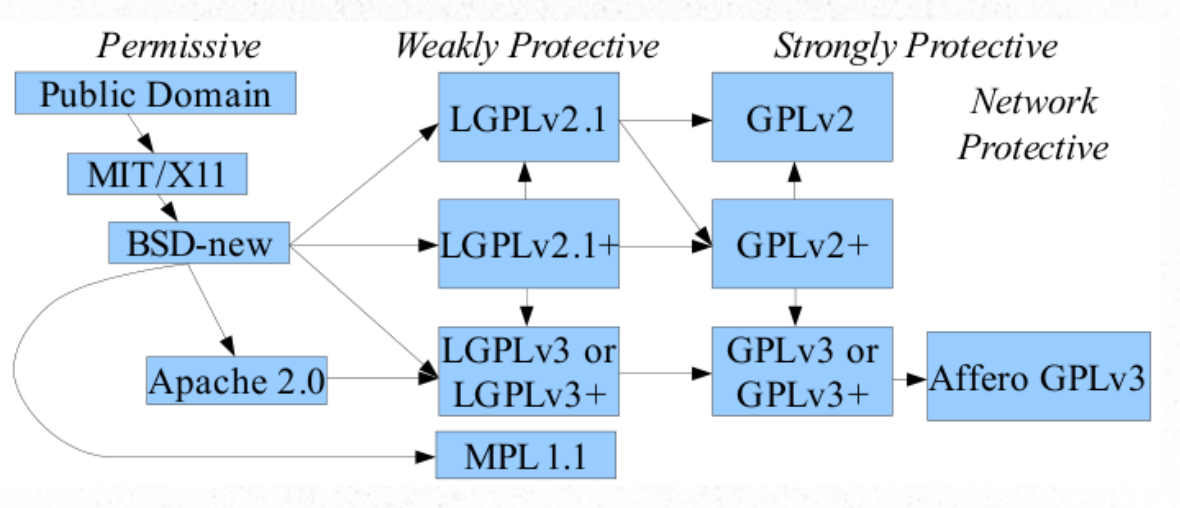
\includegraphics[width=100mm]{images/license-compatibility.png}
\caption{Mappa di compatibilità delle licenze}
\end{figure}